\documentclass[
  jou,
  longtable,
  nolmodern,
  notxfonts,
  notimes,
  mask,
  colorlinks=true,linkcolor=blue,citecolor=blue,urlcolor=blue]{apa7}

\usepackage{amsmath}
\usepackage{amssymb}




\RequirePackage{longtable}
\RequirePackage{threeparttablex}

\makeatletter
\renewcommand{\paragraph}{\@startsection{paragraph}{4}{\parindent}%
	{0\baselineskip \@plus 0.2ex \@minus 0.2ex}%
	{-.5em}%
	{\normalfont\normalsize\bfseries\typesectitle}}

\renewcommand{\subparagraph}[1]{\@startsection{subparagraph}{5}{0.5em}%
	{0\baselineskip \@plus 0.2ex \@minus 0.2ex}%
	{-\z@\relax}%
	{\normalfont\normalsize\bfseries\itshape\hspace{\parindent}{#1}\textit{\addperi}}{\relax}}
\makeatother




\usepackage{longtable, booktabs, multirow, multicol, colortbl, hhline, caption, array, float, xpatch}
\setcounter{topnumber}{2}
\setcounter{bottomnumber}{2}
\setcounter{totalnumber}{4}
\renewcommand{\topfraction}{0.85}
\renewcommand{\bottomfraction}{0.85}
\renewcommand{\textfraction}{0.15}
\renewcommand{\floatpagefraction}{0.7}

\usepackage{tcolorbox}
\tcbuselibrary{listings,theorems, breakable, skins}
\usepackage{fontawesome5}

\definecolor{quarto-callout-color}{HTML}{909090}
\definecolor{quarto-callout-note-color}{HTML}{0758E5}
\definecolor{quarto-callout-important-color}{HTML}{CC1914}
\definecolor{quarto-callout-warning-color}{HTML}{EB9113}
\definecolor{quarto-callout-tip-color}{HTML}{00A047}
\definecolor{quarto-callout-caution-color}{HTML}{FC5300}
\definecolor{quarto-callout-color-frame}{HTML}{ACACAC}
\definecolor{quarto-callout-note-color-frame}{HTML}{4582EC}
\definecolor{quarto-callout-important-color-frame}{HTML}{D9534F}
\definecolor{quarto-callout-warning-color-frame}{HTML}{F0AD4E}
\definecolor{quarto-callout-tip-color-frame}{HTML}{02B875}
\definecolor{quarto-callout-caution-color-frame}{HTML}{FD7E14}

%\newlength\Oldarrayrulewidth
%\newlength\Oldtabcolsep


\usepackage{hyperref}




\providecommand{\tightlist}{%
  \setlength{\itemsep}{0pt}\setlength{\parskip}{0pt}}
\usepackage{longtable,booktabs,array}
\usepackage{calc} % for calculating minipage widths
% Correct order of tables after \paragraph or \subparagraph
\usepackage{etoolbox}
\makeatletter
\patchcmd\longtable{\par}{\if@noskipsec\mbox{}\fi\par}{}{}
\makeatother
% Allow footnotes in longtable head/foot
\IfFileExists{footnotehyper.sty}{\usepackage{footnotehyper}}{\usepackage{footnote}}
\makesavenoteenv{longtable}

\usepackage{graphicx}
\makeatletter
\newsavebox\pandoc@box
\newcommand*\pandocbounded[1]{% scales image to fit in text height/width
  \sbox\pandoc@box{#1}%
  \Gscale@div\@tempa{\textheight}{\dimexpr\ht\pandoc@box+\dp\pandoc@box\relax}%
  \Gscale@div\@tempb{\linewidth}{\wd\pandoc@box}%
  \ifdim\@tempb\p@<\@tempa\p@\let\@tempa\@tempb\fi% select the smaller of both
  \ifdim\@tempa\p@<\p@\scalebox{\@tempa}{\usebox\pandoc@box}%
  \else\usebox{\pandoc@box}%
  \fi%
}
% Set default figure placement to htbp
\def\fps@figure{htbp}
\makeatother


% definitions for citeproc citations
\NewDocumentCommand\citeproctext{}{}
\NewDocumentCommand\citeproc{mm}{%
  \begingroup\def\citeproctext{#2}\cite{#1}\endgroup}
\makeatletter
 % allow citations to break across lines
 \let\@cite@ofmt\@firstofone
 % avoid brackets around text for \cite:
 \def\@biblabel#1{}
 \def\@cite#1#2{{#1\if@tempswa , #2\fi}}
\makeatother
\newlength{\cslhangindent}
\setlength{\cslhangindent}{1.5em}
\newlength{\csllabelwidth}
\setlength{\csllabelwidth}{3em}
\newenvironment{CSLReferences}[2] % #1 hanging-indent, #2 entry-spacing
 {\begin{list}{}{%
  \setlength{\itemindent}{0pt}
  \setlength{\leftmargin}{0pt}
  \setlength{\parsep}{0pt}
  % turn on hanging indent if param 1 is 1
  \ifodd #1
   \setlength{\leftmargin}{\cslhangindent}
   \setlength{\itemindent}{-1\cslhangindent}
  \fi
  % set entry spacing
  \setlength{\itemsep}{#2\baselineskip}}}
 {\end{list}}
\usepackage{calc}
\newcommand{\CSLBlock}[1]{\hfill\break\parbox[t]{\linewidth}{\strut\ignorespaces#1\strut}}
\newcommand{\CSLLeftMargin}[1]{\parbox[t]{\csllabelwidth}{\strut#1\strut}}
\newcommand{\CSLRightInline}[1]{\parbox[t]{\linewidth - \csllabelwidth}{\strut#1\strut}}
\newcommand{\CSLIndent}[1]{\hspace{\cslhangindent}#1}


\usepackage[nolongtablepatch]{lineno}
\linenumbers



\usepackage{newtx}

\defaultfontfeatures{Scale=MatchLowercase}
\defaultfontfeatures[\rmfamily]{Ligatures=TeX,Scale=1}





\title{\textbf{Measuring Depression and Anxiety with 4 items? Adaptation
of the PHQ-4 to increase its Sensitivity to Subclinical Variability}}


\shorttitle{Adaptation of the PHQ-4}


\usepackage{etoolbox}









\authorsnames[{1,2},{3},{1},{3,4,5}]{Dominique Makowski,An Shu Te,Ana
Neves,S.H. Annabel Chen}







\authorsaffiliations{
{School of Psychology, University of Sussex},{Sussex Centre for
Consciousness Science, University of Sussex},{School of Social
Sciences, Nanyang Technological University},{LKC Medicine, Nanyang
Technological University},{Centre for Research and Development in
Learning, Nanyang Technological University}}




\leftheader{Makowski, Te, Neves and Chen}



\abstract{The PHQ-4 is an ultra-brief (4 items) screening questionnaire
for depression and anxiety. In this brief report, we test the benefits
of adding one additional response option (``Once or twice'', in between
``Not at all'' and ``Several days'') to improve the scale's sensitivity
to milder alterations, and thus increase its usefulness in subclinical
populations. In study 1 (N=485), we provide evidence using Item Response
Theory (IRT) that the new response option does improve the scale's
psychometric quality and extends the sensitivity to the measured
constructs on the lower end of the spectrum. In study 2 (N=836), we show
that the refined version offers an improved sensitivity to subclinical
variability in depression (indexed by the BDI-II) as compared to the
original version. In conclusion, adding the ``once or twice'' response
option is a low-cost way of increasing the PHQ-4's sensitivity to
subclinical variability, making it a tool of choice for general
population research.}

\keywords{PHQ-4, depression, anxiety, brief questionnaire validation,
ultra short scale}

\authornote{\par{\addORCIDlink{Dominique
Makowski}{0000-0001-5375-9967}}\par{\addORCIDlink{An Shu
Te}{0000-0002-9312-5552}}\par{\addORCIDlink{Ana
Neves}{0009-0006-0020-7599}}\par{\addORCIDlink{S.H. Annabel
Chen}{0000-0002-1540-5516}} 
\par{ }
\par{     \begin{tcolorbox}[enhanced jigsaw, colback=white, toprule=.15mm, opacityback=0, arc=.35mm, breakable, bottomrule=.15mm, colframe=quarto-callout-note-color-frame, rightrule=.15mm, left=2mm, leftrule=.75mm]

This preprint is a non-peer-reviewed work from the
\href{https://realitybending.github.io/}{\textbf{Reality Bending Lab}}.
\begin{center}

\includegraphics[width=0.2\linewidth,height=\textheight,keepaspectratio]{manuscript_files/mediabag/ReBeL_LogoOnly_hu114.png}
\end{center}

\end{tcolorbox}  Author roles were classified using the Contributor Role Taxonomy (CRediT; https://credit.niso.org/) as follows: Dominique
Makowski:   Conceptualization, Data curation, Formal Analysis, Funding
acquisition, Investigation, Methodology, Project
administration, Resources, Software, Supervision, Validation, Visualization, Writing
-- original draft; An Shu Te:   Project
administration, Resources, Writing -- original draft; Ana Neves:   Data
curation, Formal Analysis, Writing -- original draft, Writing -- review
\& editing; S.H. Annabel Chen:   Project
administration, Supervision, Writing -- review \& editing}
\par{Correspondence concerning this article should be addressed
to Dominique Makowski, Email: D.Makowski@sussex.ac.uk}
}

\usepackage{pbalance} 
\usepackage{float}
\makeatletter
\let\oldtpt\ThreePartTable
\let\endoldtpt\endThreePartTable
\def\ThreePartTable{\@ifnextchar[\ThreePartTable@i \ThreePartTable@ii}
\def\ThreePartTable@i[#1]{\begin{figure}[!htbp]
\onecolumn
\begin{minipage}{0.5\textwidth}
\oldtpt[#1]
}
\def\ThreePartTable@ii{\begin{figure}[!htbp]
\onecolumn
\begin{minipage}{0.5\textwidth}
\oldtpt
}
\def\endThreePartTable{
\endoldtpt
\end{minipage}
\twocolumn
\end{figure}}
\makeatother


\makeatletter
\let\endoldlt\endlongtable		
\def\endlongtable{
\hline
\endoldlt}
\makeatother

\newenvironment{twocolumntable}% environment name
{% begin code
\begin{table*}[!htbp]%
\onecolumn%
}%
{%
\twocolumn%
\end{table*}%
}% end code

\urlstyle{same}



\makeatletter
\@ifpackageloaded{tcolorbox}{}{\usepackage[skins,breakable]{tcolorbox}}
\@ifpackageloaded{fontawesome5}{}{\usepackage{fontawesome5}}
\definecolor{quarto-callout-color}{HTML}{909090}
\definecolor{quarto-callout-note-color}{HTML}{0758E5}
\definecolor{quarto-callout-important-color}{HTML}{CC1914}
\definecolor{quarto-callout-warning-color}{HTML}{EB9113}
\definecolor{quarto-callout-tip-color}{HTML}{00A047}
\definecolor{quarto-callout-caution-color}{HTML}{FC5300}
\definecolor{quarto-callout-color-frame}{HTML}{acacac}
\definecolor{quarto-callout-note-color-frame}{HTML}{4582ec}
\definecolor{quarto-callout-important-color-frame}{HTML}{d9534f}
\definecolor{quarto-callout-warning-color-frame}{HTML}{f0ad4e}
\definecolor{quarto-callout-tip-color-frame}{HTML}{02b875}
\definecolor{quarto-callout-caution-color-frame}{HTML}{fd7e14}
\makeatother
\makeatletter
\@ifpackageloaded{caption}{}{\usepackage{caption}}
\AtBeginDocument{%
\ifdefined\contentsname
  \renewcommand*\contentsname{Table of contents}
\else
  \newcommand\contentsname{Table of contents}
\fi
\ifdefined\listfigurename
  \renewcommand*\listfigurename{List of Figures}
\else
  \newcommand\listfigurename{List of Figures}
\fi
\ifdefined\listtablename
  \renewcommand*\listtablename{List of Tables}
\else
  \newcommand\listtablename{List of Tables}
\fi
\ifdefined\figurename
  \renewcommand*\figurename{Figure}
\else
  \newcommand\figurename{Figure}
\fi
\ifdefined\tablename
  \renewcommand*\tablename{Table}
\else
  \newcommand\tablename{Table}
\fi
}
\@ifpackageloaded{float}{}{\usepackage{float}}
\floatstyle{ruled}
\@ifundefined{c@chapter}{\newfloat{codelisting}{h}{lop}}{\newfloat{codelisting}{h}{lop}[chapter]}
\floatname{codelisting}{Listing}
\newcommand*\listoflistings{\listof{codelisting}{List of Listings}}
\makeatother
\makeatletter
\makeatother
\makeatletter
\@ifpackageloaded{caption}{}{\usepackage{caption}}
\@ifpackageloaded{subcaption}{}{\usepackage{subcaption}}
\makeatother

% From https://tex.stackexchange.com/a/645996/211326
%%% apa7 doesn't want to add appendix section titles in the toc
%%% let's make it do it
\makeatletter
\xpatchcmd{\appendix}
  {\par}
  {\addcontentsline{toc}{section}{\@currentlabelname}\par}
  {}{}
\makeatother

%% Disable longtable counter
%% https://tex.stackexchange.com/a/248395/211326

\usepackage{etoolbox}

\makeatletter
\patchcmd{\LT@caption}
  {\bgroup}
  {\bgroup\global\LTpatch@captiontrue}
  {}{}
\patchcmd{\longtable}
  {\par}
  {\par\global\LTpatch@captionfalse}
  {}{}
\apptocmd{\endlongtable}
  {\ifLTpatch@caption\else\addtocounter{table}{-1}\fi}
  {}{}
\newif\ifLTpatch@caption
\makeatother

\begin{document}

\maketitle


\setcounter{secnumdepth}{-\maxdimen} % remove section numbering

\setlength\LTleft{0pt}

\resetlinenumber[1]

The Patient Health Questionnaire-4 (PHQ-4) is an ultra brief measurement
of core signs of depression and anxiety
(\citeproc{ref-kroenke2009ultra}{Kroenke et al., 2009}). It consists of
two items for depression (PHQ--2,
\citeproc{ref-kroenke2003patient}{Kroenke et al., 2003}) and anxiety
(GAD--2, \citeproc{ref-kroenke2007anxiety}{Kroenke et al., 2007}), each
corresponding to DSM-5 diagnostic symptoms for major depressive disorder
(MDD) and generalized anxiety disorder (GAD). It has been validated
across many languages and populations
(\citeproc{ref-christodoulaki2022validation}{Christodoulaki et al.,
2022}; \citeproc{ref-materu2020psychometric}{Materu et al., 2020};
\citeproc{ref-mendoza2022factor}{Mendoza et al., 2022}), becoming one of
the most popular screening instruments for depression and anxiety
(\citeproc{ref-maurer2018depression}{Maurer et al., 2018}).

While the scale has been validated and used in the general population
and non-clinical samples (\citeproc{ref-hajek2020prevalence}{Hajek \&
König, 2020}; \citeproc{ref-lowe20104}{Löwe et al., 2010}), its initial
purpose was to reliably discriminate and identify potential MDD/GAD
patients. This discriminative goal materializes in the scale's design
and the existence of categorical cut-offs, which does not necessarily
entail a focus on the sensitivity to milder mood alterations. In
particular, the gap between the two lowest possible answers, ``Not at
all'' and ``Several days'', is quite large and possibly leaves out the
possibility of more subtle occurrences. While this is not necessarily an
issue in clinical and diagnostic contexts, it might lead to a
sub-optimal discrimination of affective levels on the lower end of the
spectrum, important for instance in the context of subclinical
variability quantification.

\textbf{Enabling a more precise assessment of low-severity alterations
is important, as milder symptoms are significant predictors of future
clinical disorders and are associated with present functional
impairments and reduced quality of life
(\citeproc{ref-cuijpers2004subthreshold}{Cuijpers \& Smit, 2004};
\citeproc{ref-judd1998major}{Judd et al., 1998}). In addition, the
growing reliance on large-scale, often online, psychological and
epidemiological surveys, to monitor population-level mental health,
evaluate interventions, or track responses to global stressors such as
pandemics or geopolitical crises, demands tools that are both brief and
sensitive to small but meaningful fluctuations.}

This brief report aims at testing the possibility of enhancing - with
minimal changes to the original scale - the PHQ-4 sensitivity to mild
mood level inflections. In the first study, we will evaluate whether the
new response option is prevalently used by participants, and whether it
does capture a specific part of the construct. In the second study, we
will compare the refined PHQ-4 version to the original one in terms of
sensitivity to subclinical variability in depression, using the Beck
Depression Inventory (BDI-II, \citeproc{ref-beck1996beck}{Beck et al.,
1996}) and the Trait scale of the State-Trait Anxiety Inventory (STAI-5,
\citeproc{ref-zsido2020development}{Zsido et al., 2020}) as our
ground-truth measures of depression and anxiety.

\section{Study 1}\label{study-1}

\subsection{Method}\label{method}

\subsubsection{Participants}\label{participants}

The sample consists of 485 English-speaking participants (Mean age =
30.1 \(\pm\) 10.1 {[}18, 73{]}; 50.3\% females) from the general
population recruited via \emph{Prolific}, a crowd-sourcing platform
recognized for providing high quality data
(\citeproc{ref-peer2022data}{Peer et al., 2022}). The only inclusion
criterion was a fluent proficiency in English to ensure that the task
instructions would be well-understood. This study was approved by the
NTU Institutional Review Board (NTU IRB-2022-187). All participants
provided their informed consent prior to participation and were
incentivized after completing the study.

\subsubsection{Measures}\label{measures}

In the original PHQ-4, the instructions \emph{``Over the last 2 weeks,
how often have you been bothered by the following problems?''} are
followed with 4 items (A1 - \emph{Feeling nervous, anxious or on edge};
A2 - \emph{Not being able to stop or control worrying}; D1 -
\emph{Little interest or pleasure in doing things}; D2 - \emph{Feeling
down, depressed, or hopeless}). The original answer options are ``Not at
all'' (0), ``Several days'' (1), ``More than half the days'' (2),
``Nearly every day'' (3). The total score is computed by summing the
responses of each facet resulting in a 0-6 score for depression and
anxiety.

For the refined version, we added a ``Once or twice'' option between
``Not at all'' and ``Several days''in order to better capture potential
mild mood inflections (see \citeproc{ref-dobson1979equidistant}{Dobson
\& Mothersill, 1979} for the choice of the label).

\subsubsection{Procedure}\label{procedure}

Participants were administered the refined PHQ-4 online as part of
another study, which contained additional questionnaires and tasks not
relevant fort the current analysis. The PHQ-4 was presented in a
randomized order with other questionnaires. The data is available in
open-access at
https://github.com/RealityBending/IllusionGameReliability.

\subsection{Results}\label{results}

The analysis was carried out using \emph{R 4.4}
(\citeproc{ref-RCoreTeam}{R Core Team, 2023}), the \emph{tidyverse}
(\citeproc{ref-wickham2019welcome}{Wickham et al., 2019}), and the
\emph{easystats} collection of packages
(\citeproc{ref-ludecke2019insight}{Lüdecke et al., 2019},
\citeproc{ref-ludecke2020extracting}{2020},
\citeproc{ref-ludecke2021performance}{2021};
\citeproc{ref-patil2022datawizard}{Patil et al., 2022}). All
reproducible scripts and complimentary analyses are available
open-access at https://github.com/DominiqueMakowski/PHQ4R

\begin{figure*}[!htbp]

{\caption{{A) Proportion of answers of each type to the four items. B)
Prevalence of answer pairs. C) Item Information Curves from IRT showing
the coverage by each item and response of the latent dimension.
Typically, an optimally informative item would display a large coverage
over theta, with each response presenting a narrow coverage (high
discrimination between different levels).}{\label{fig-one}}}}

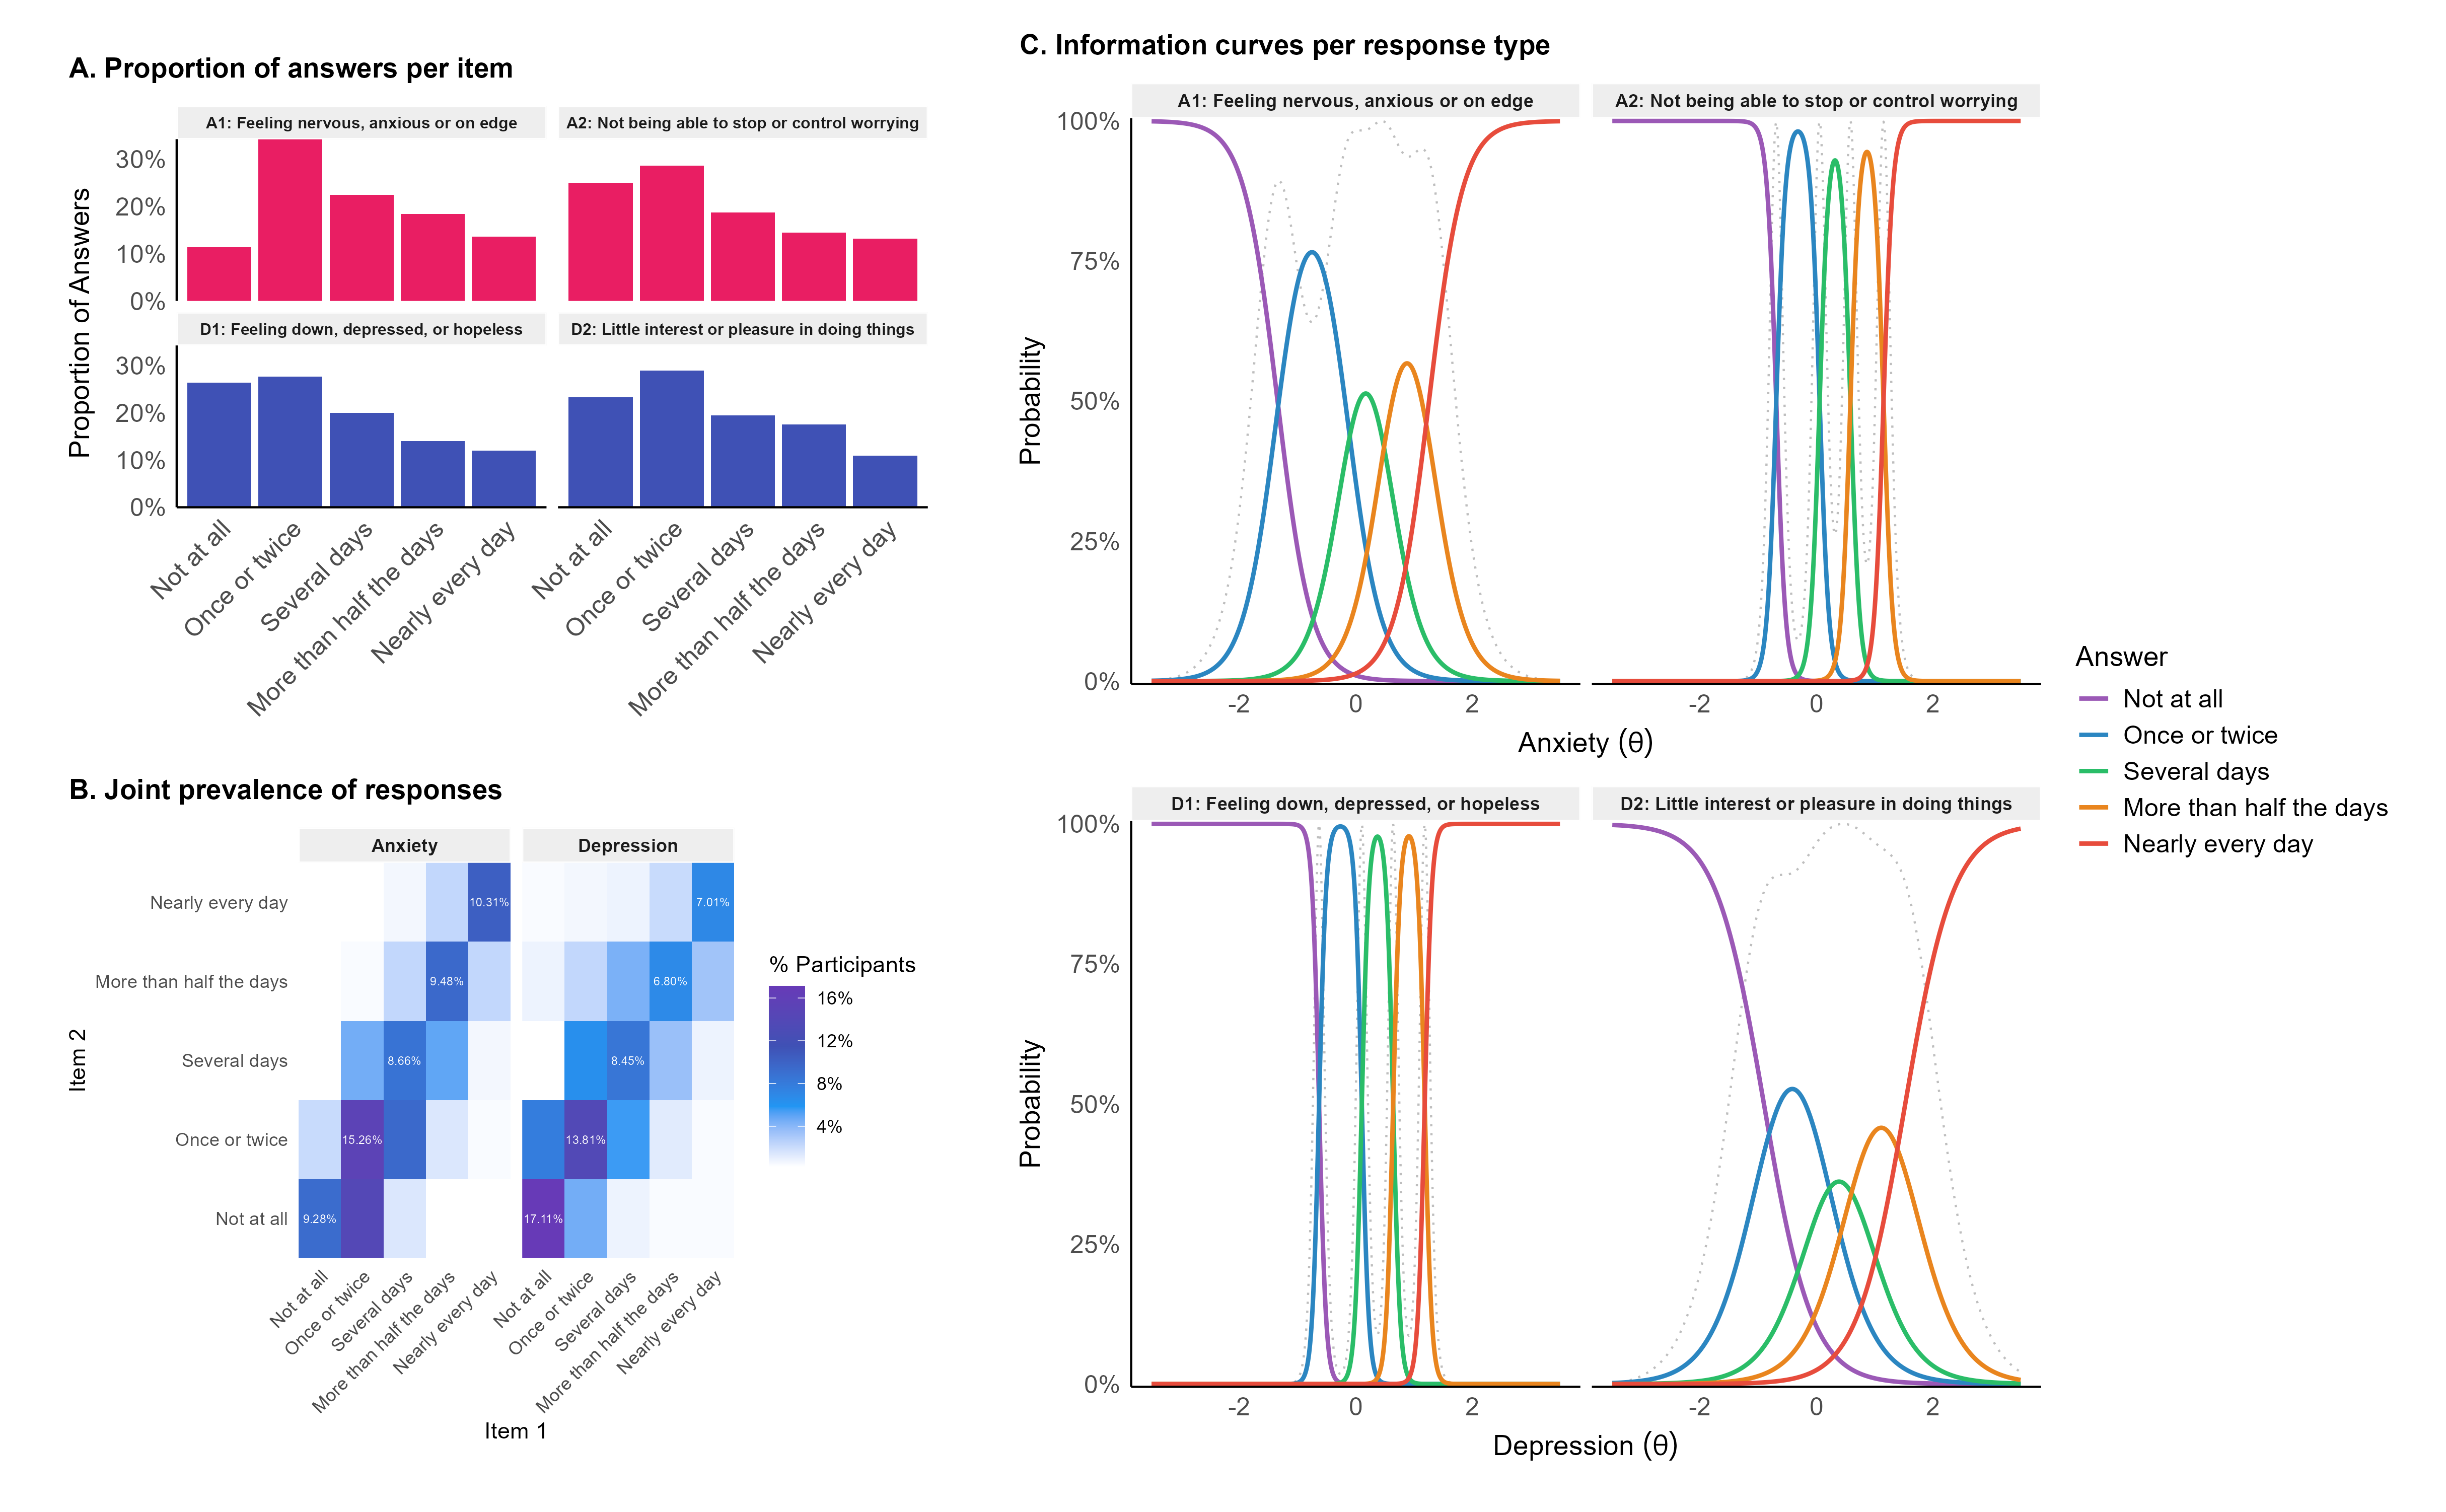
\includegraphics[width=1\linewidth,height=\textheight,keepaspectratio]{../../study1/figures/figure1.png}

\end{figure*}

\subsubsection{Descriptive Statistics}\label{descriptive-statistics}

The consistency of the anxiety (\(Cronbach's~\alpha = 0.903\)) and
depression (\(Cronbach's~\alpha = 0.841\)) subscales is excellent
(responses were treated as ordinal). The proportion of response types
stratified by item (see Figure~\ref{fig-one}) shows that the new ``Once
or twice'' option was the most prevalent response for all items (on
average selected in 29.12\% of cases).

\subsubsection{Item Response Theory}\label{item-response-theory}

Item Response Theory (IRT) provides insights into how well items and
responses capture an underlying latent trait \(\theta\). For each of the
subscales, we fitted a unidimensional graded response model (GRM,
\citeproc{ref-samejima1997graded}{Samejima, 1997}). For anxiety, the
latent anxiety dimension (\(\theta_{anxiety}\)) captured 89.2\% of the
total variance across the two items (RMSEA = 0.031). The discrimination
parameters suggested that the first item was less precise
(\(\alpha = 3.42\)) than the second item (\(\alpha = 12.55\)) in its
ability to discriminate between various levels of anxiety (i.e., each
response on the second item covers a more exclusive range of
\(\theta_{anxiety}\), as can be seen in Figure~\ref{fig-one}). The
latent depression trait (\(\theta_{depression}\)) The two depression
items captured 82.8\% of the total variance across the two items (RMSEA
= 0.044), and the opposite pattern was found: the first item had a
higher precision (\(\alpha = 16.46\)) than the second
(\(\alpha = 2.41\)). However, it is important to note that the ``less
precise'' items were also the ones covering a larger portion of the
latent space (being more sensitive especially on the lower end of the
spectrum), offering an interesting trade-off between sensitivity and
precision. Most importantly for our objective, the added ``Once or
twice'' option did cover a selective and unique portion of the latent
space.

\subsection{Discussion}\label{discussion}

The fact that the new ``Once or twice'' response option was the most
prevalent response speaks to its usefulness in capturing more accurately
participants' expression. The IRT analysis further revealed that this
response tracks with precision a unique portion of the variability in
the latent factors measured by the instrument. Taken together, our
results suggest that adding this option response increases the scale's
potential to discriminate average mood levels (which are superior to
zero) from lower-end extremes (the true zero).

\textbf{One natural methodological limitation pertains to the
application of the IRT framework to pairs of items. While this is
statistically sound (the graded model utilizes the full response pattern
information and does not solely rely on the item covariance matrix for
parameter estimation), it is important to underline that in our study's
context, ``the latent anxiety/depression dimension'' merely corresponds
to the amalgamation of the two items of the anxiety or depression
subscale, and not to a more general and independent latent anxiety or
depression factor.}

\textbf{In summary, the main take-away of this first study is that the
``Once or twice'' response option appears as a popular choice, which
begs the question of its usefulness in capturing more fine-grained
variations of the underlying dimensions as measured by independent
tools.}

\section{Study 2}\label{study-2}

\subsection{Method}\label{method-1}

\subsubsection{Participants}\label{participants-1}

The initial sample consisted of 1053 participants, recruited (181 were
recruited on \emph{Prolific}, 772 students from the University of Sussex
via \emph{SONA}, and the rest through convenience sampling as part of
dissertation students' data collection). We used attention checks as the
primary target for participant exclusion. We excluded 194 participants
(18.42\%) for failing at least one attention check, and 23 (2.18\%) that
were outliers (\(|z_{robust}| > 2.58\)) on measures significantly
related to the probability of failing attention checks (namely, the
standard deviation of all the items of the Interoceptive Accuracy Scale,
as well as the the multivariate distance obtained with the OPTICS
algorithm, see \citeproc{ref-theriault2024check}{Thériault et al.,
2024}). The experiment duration was not related to the probability of
failing attention checks and was thus not used as an exclusion
criterion.

The final sample included 836 participants (Mean age = 25.1 \(\pm\) 11.3
{[}18, 76{]}; 73.8\% women). This study was approved by the University
of Sussex' Ethics Committee (ER/ASF25/4).

In this sample, 51 participants (6.10\%) were coded as having
Depression, as indexed by the self-reported presence of MDD together
with the use of a treatment (antidepressent, anxiolytic and/or therapy),
and 87 participants (10.41\%) were coded as having Anxiety, as indexed
by the self-reported presence of GAD or Panic Disorder, also together
with the use of a treatment.

\subsubsection{Measures}\label{measures-1}

Participants were randomly assigned to complete either the original or
refined version of the PHQ-4, which included one additional response
option (``Once or twice''). \textbf{To preserve comparability with the
original PHQ-4 scoring system and avoid altering the scale's total score
range or established cut-off thresholds, we assigned the new response
option a value of 0.5, placing it midway between ``Not at all'' (0) and
``Several days'' (1). While this scoring assumes equal spacing between
response options - a common but imperfect convention in ordinal scales -
it offers a pragmatic compromise between conceptual fidelity and applied
utility.}

Beck's Depression Inventory (BDI-II, \citeproc{ref-beck1996beck}{Beck et
al., 1996}) was used as a ground truth measure of depressive symptoms.
It includes 21 items, each addressing a specific depression symptom and
offering four response options scored from 0 to 3. Participants are
instructed to select the option that best describes how they have felt
over the past two weeks. The total score is calculated by summing the
scores for all 21 items, with higher scores indicating greater severity
of depressive symptoms.

The short version of the trait subscale of the State-Trait Anxiety
Inventory (STAI-5, \citeproc{ref-zsido2020development}{Zsido et al.,
2020}) was used as a ground truth measure of anxiety. This abridged
version of the STAI (\citeproc{ref-spielberger1970manual}{Spielberger,
1970}) includes 5 items rated on a 4-point Likert scale. Changes were
made in the instructions from asking \emph{``how participants feel right
now''} to \emph{``over the past 2 weeks''} to keep it consistent with
the instructions of the PHQ-4 and BDI-II. A general score of anxiety was
computed by averaging all the items.

Participants were also asked to complete two questionnaires of
interoception, namely the Interoceptive Accuracy Scale (IAS, 21 items
rated on analog scales, \citeproc{ref-murphy2020testing}{Murphy et al.,
2020}) and the Multidimensional Assessment of Interoceptive Awareness
(MAIA-2 - 37 items, \citeproc{ref-mehling2018multidimensional}{Mehling
et al., 2018}).

After demographic questions, participants were asked to report the
current presence of psychiatric issues (from a list), as well as the
usage of treatment (antidepressants, mood stabilizers, anxiolytics,
therapy). We indexed the presence of a depression when participants
reported suffering from either Major Depressive Disorder (MDD) or
Dysthymia, as well as undergoing a medical treatment. Similarly, we
indexed the presence of an anxiety disorder when participants reported
suffering from either Generalized Anxiety Disorder (GAD) or Panic
Disorder, as well as undergoing a medical treatment.

\subsubsection{Procedure}\label{procedure-1}

The original or refined version of the PHQ-4 was followed by the BDI-II,
STAI-5, IAS, and MAIA-2, presented in random order. The IAS
(\citeproc{ref-murphy2020testing}{Murphy et al., 2020}) and the MAIA-2
(\citeproc{ref-mehling2018multidimensional}{Mehling et al., 2018}) were
included as part of another focused on interoception, and were only used
in this study as part of data quality control checks.

\subsection{Results}\label{results-1}

As all the scripts, analysis details and results tables are available
open-access at https://github.com/DominiqueMakowski/PHQ4R, we will focus
on reporting the main results.

\begin{figure*}[!htbp]

{\caption{{A) PHQ-4 depression and anxiety scores against their
respective ground-truth measures, the BDI-22 and the STAI-5. Bayes
factors in grey tell if there is a difference, for the same PHQ-4 score,
between the original and the refined version (BFs \textless{} 1 suggest
no difference and thus evidence for a comparability of the refined
version with respect fo the original scale. Bayes factors in yellow
represent how new in-between scores (0.5, 1.5, 2.5, \ldots) available
with refined version differ from the adjacent scores (BFs \textgreater{}
3 suggest that half a point of difference on the refined PHQ-4 relates
to a significant difference on the ground truth measure). BF \textless{}
1/3°, BF \textgreater{} 3*, BF \textgreater{} 10**, BF \textgreater{}
30***. B) Bootstrapped distributions of the difference of correlation
between the revised PHQ-4 scores and the original one for sub-clinical
threshold scores of depression and anxiety. Positive differences suggest
that the correlation between the ground-truth measure and the refined
PHQ-4 score was stronger compared to the original version. C) Predictive
power of the PHQ-4 scores on the presence of a depression or anxiety
disorder. The upper plots show the relationship modelled by a logistic
regression, while the above plots represent the ROC curves (in which a
line further away from the diagonal represents a higher combination of
sensitivity and specificity).}{\label{fig-two}}}}

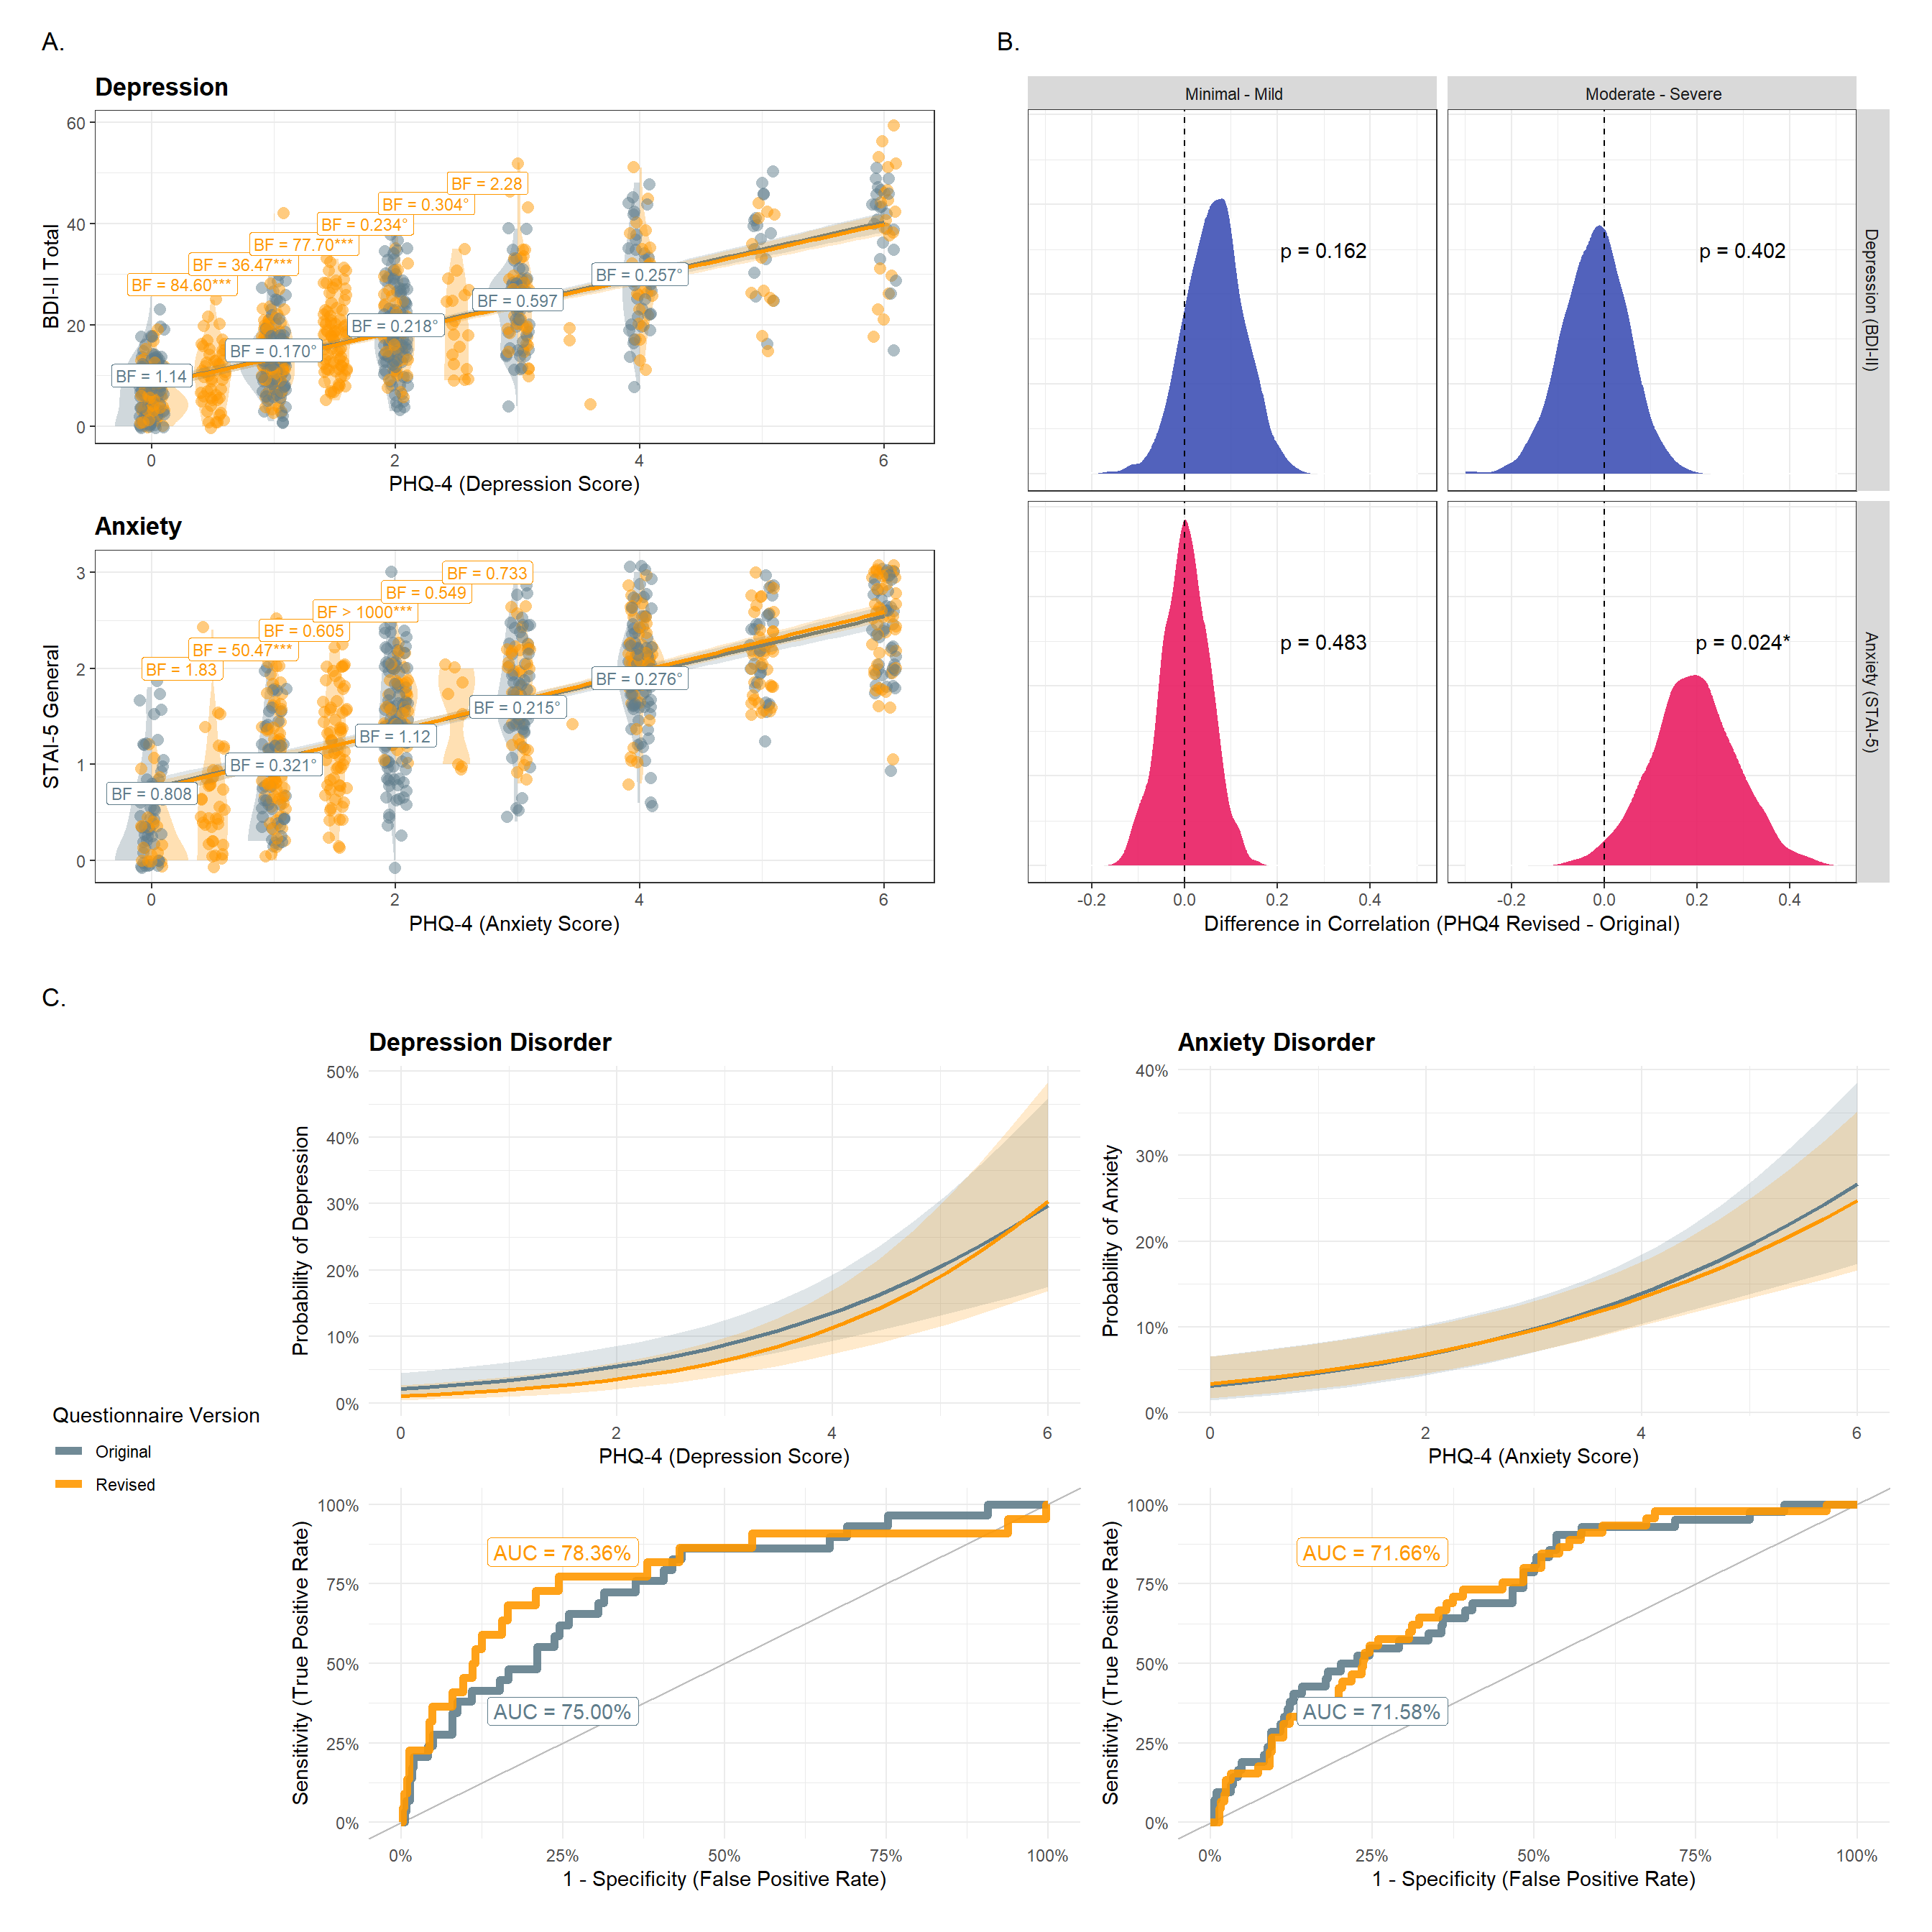
\includegraphics[width=1\linewidth,height=\textheight,keepaspectratio]{../../study2/analysis/2_analysis_files/figure-html/figure-1.png}

\end{figure*}

\subsubsection{\texorpdfstring{PHQ-4 Depression \emph{vs.}
BDI-II}{PHQ-4 Depression vs. BDI-II}}\label{phq-4-depression-vs.-bdi-ii}

\textbf{A linear model testing the interaction effect \(\Delta\) of the
refined condition on the intercept (representing by how much the value
of the outcome when the PHQ score is 0 changes for the refined version
compared the original) and slope (its increase or decrease by the
refined version compared to the original) of the relationship between
the PHQ-4 depression score and the BDI-II total score was fitted.} The
model predicting the BDI-II total score with the PHQ-4 depression score
showed no interaction related to the PHQ-4 version
(\(\Delta Intercept_{\text{refined}} =  -0.13,~95\%~CI~[-1.73, 1.47],~t(832) =  -0.16,~p = 0.871\);
\(\Delta \beta_{\text{refined}} = -0.05,~95\%~CI~[-0.70, 0.60],~t(832) = -0.15,~p = 0.883\)),
suggesting no differences in the relationship pattern between the two
versions (see Figure~\ref{fig-two}).

Moreover, Bayesian \emph{t}-tests (using \emph{BayesFactor}'s
\texttt{ttestBF()} function with default priors,
\citeproc{ref-moreyrouder2024}{Morey \& Rouder, 2024}) comparing the
BDI-II scores between the refined and the original version at each
integer score (0, 1, 2, 3) yielded no evidence in favour of a
significant difference (BF \textgreater{} 3). In other words, having the
same score on the refined version as on the original version was related
to the same outcome on the BDI-II.

However, the low in-between scores from the refined version are overall
capturing significantly different levels of depression compared to the
adjacent scores. Scoring 0.5 was associated with a higher BDI-II score
than scoring 0 (BF \textgreater{} 30), and lower scores than scoring 1
(BF \textgreater{} 30). Similarly, scoring 1.5 was associated with a
higher BDI-II score than scoring 1 (BF \textgreater{} 30), but not lower
scores than scoring 2 (BF = 0.234).

\subsubsection{\texorpdfstring{PHQ-4 Anxiety \emph{vs.}
STAI-5}{PHQ-4 Anxiety vs. STAI-5}}\label{phq-4-anxiety-vs.-stai-5}

The linear regression predicting the STAI-5 general score with the PHQ-4
anxiety score showed no interaction related to the PHQ-4 version
(\(\Delta Intercept_{\text{refined}} =  -0.02,~95\%~CI~[-0.15, 0.11],~t(832) =  -0.32,~p = 0.750\);
\(\Delta \beta_{\text{refined}} = 0.01,~95\%~CI~[-0.03, 0.05],~t(832) = 0.56,~p = 0.576\)),
suggesting no differences in the relationship pattern between the two
versions.

Moreover, Bayesian \emph{t}-tests comparing the STAI-5 scores between
the refined and the original version at each integer score yielded no
evidence in favour of a significant difference. In other words, having
the same score on the refined version as on the original version was
related to the same outcome on the STAI-5.

However, comparing in-between scores with adjacent scores yielded mixed
results. Scoring 0.5 on the PHQ-4 anxiety was not significantly
associated with a different level of STAI-5 compared to scoring 0 (BF =
1.83), but was with scores of 1 (BF \textgreater{} 30). Similarly, there
was no evidence that scoring 1.5 was different from scoring 1 (BF =
0.605), but strong evidence that it was different from scoring 2 (BF
\textgreater{} 30).

\subsubsection{Correlation Differences}\label{correlation-differences}

While the relationship pattern (i.e., the slope of the linear
relationship) was not affected by the PHQ-4 version, we focused next on
testing the difference in the strength (i.e., the precision) of the
relationship, in particular at the lower end of the spectrum (i.e., for
sub-clinical threshold scores of the BDI-II and STAI-5). We bootstrapped
(2000 iterations) the difference in correlation between the refined and
the original version for each of the two ground-truth measures,
separately for the BDI-II subsamples (minimal to mild \textless= 18;
moderate to severe \textgreater{} 18) and the STAI-5 subsamples (minimal
to mild \textless{} 2; moderate to severe \textgreater= 2).

The results suggested that in the subclinical range of the BDI-II, the
correlation between its score and the PHQ-4 Depression score was
marginally higher (although not significantly,
\(p_{one-sided} = 0.164\)) for the refined version compared to the
original one. No correlation differences were observed in the moderate
to severe range of the BDI-II.

For the STAI-5, there was no difference in the correlation between the
refined and the original version in the subclinical range of the STAI-5.
Surprisingly, we observed a stronger correlation between the refined
PHQ-4 Anxiety score and the STAI-5 in the moderate to severe range
compared to the original version (\(p_{one-sided} = 0.017\)).

\subsubsection{Predictive Power}\label{predictive-power}

Finally, we tested the predictive power of the PHQ-4 depression and
anxiety scores on the presence of a depression or anxiety disorder,
respectively. We modeled the relationship with a logistic regression.
While the PHQ-4 was overall a strong predictor of the outcome, there was
no significant difference between the two PHQ-4 versions.

However, the ROC curves for the refined and the original version of the
PHQ-4, suggested that the refined version had a better sensitivity /
specificity trade-off (AUC = 78.36\%) compared to the original version
(AUC=75\%), in particular on the lower end of the spectrum. The
difference was negligible for anxiety.

\subsection{Discussion}\label{discussion-1}

These results suggest that the new ``Once or twice'' response option to
the PHQ-4 does help capturing more fine-grained variations of depressive
symptoms, particularly in the subclinical range. Importantly, adding
this new response option with the scoring of 0.5 does not disrupt the
quality of the scale, which scores remain comparable to that of the
original version.

The results for the anxiety subscale appear more mixed, with less
evident benefits. However, this might have been partly caused by our
design decision regarding the questionnaire used for the ground-truth
measure of anxiety. Indeed, we used the abridged version of the STAI,
which only included 5 items, arguably limiting the sensitivity of the
anxiety measure in the first place.

\textbf{One of the potential limitation of our study includes the choice
of the measures used as external ``ground-truth'' of depression and
anxiety, namely the BDI-II and the STAI-5. For instance, there is
ongoing debate about the STAI's discriminant validity (which might
extend to its short form used in the present study). A recent
meta-analysis reported that trait anxiety scores were more strongly
associated with depressive than anxiety disorders
(\citeproc{ref-knowles2020specificity}{Knowles \& Olatunji, 2020}),
suggesting that the scale may rather capture general negative affect
than specifically anxiety. Regarding the BDI-II, existing evidence that
suggests its relative lack of sensitivity for low-severity depression
(\citeproc{ref-olino2012measuring}{Olino et al., 2012}) - comparable to
similar instruments of its size (e.g., CES-D), and an improvement over
the BDI-I (\citeproc{ref-wahl2014standardization}{Wahl et al., 2014}) -
put into question its choice for our goal of showing increased
sub-clinical sensitivity. Thus, future studies should verify these
findings with alternative measures of anxiety and depression and
clinically assessed populations.}

Indeed, although we used a stricter criterion for classifying
participants as having a depression or an anxiety disorder by
restricting it to participants also reporting undergoing a medical
treatment, it was still based on self-reported data. Studies in
controlled clinical settings are needed to confirm the potential
benefits of the refined PHQ-4 in mood disorders detection accuracy.

\section{General Discussion}\label{general-discussion}

The objective of this study was to test the introduction of a ``Once or
twice'' response option to the PHQ-4 to enhance its sensitivity to
milder mood fluctuations. In the first study, we showed that the new
response option was used prevalently by participants and did capture a
unique portion of the depression and anxiety underlying dimensions. In
the second study, we showed that the refined version of the PHQ-4 was
able to better differentiate lower levels of depression compared to the
original version, while remaining comparable. Although the benefits of
this refinement appear to be fairly minor, and particularly marked for
the depression score compared to anxiety, this low-cost improvement
appear useful to implement when measuring depression and anxiety using
the PHQ-4 ultra-short screening questionnaire.

\textbf{While adding granularity to the response format appears useful
for the PHQ-4, it is possible that similar benefits could be found with
other scales and measures. While the use of a limited, highly
discriminating set of response options is understandable for specific
applications (e.g., clinical diagnosis), we recommend future studies to
investigate response format and its potential improvement for other
scales used in online surveys and general population research.}

\section{Acknowledgements}\label{acknowledgements}

We would like to thank the dissertation students from the University of
Sussex for their help in data collection.

\section{References}\label{references}

\phantomsection\label{refs}
\begin{CSLReferences}{1}{0}
\bibitem[\citeproctext]{ref-beck1996beck}
Beck, A. T., Steer, R. A., Brown, G. K., et al. (1996). \emph{Beck
depression inventory}.

\bibitem[\citeproctext]{ref-christodoulaki2022validation}
Christodoulaki, A., Baralou, V., Konstantakopoulos, G., \& Touloumi, G.
(2022). Validation of the patient health questionnaire-4 (PHQ-4) to
screen for depression and anxiety in the greek general population.
\emph{Journal of Psychosomatic Research}, \emph{160}, 110970.

\bibitem[\citeproctext]{ref-cuijpers2004subthreshold}
Cuijpers, P., \& Smit, F. (2004). Subthreshold depression as a risk
indicator for major depressive disorder: A systematic review of
prospective studies. \emph{Acta Psychiatrica Scandinavica},
\emph{109}(5), 325--331.

\bibitem[\citeproctext]{ref-dobson1979equidistant}
Dobson, K. S., \& Mothersill, K. J. (1979). Equidistant categorical
labels for construction of likert-type scales. \emph{Perceptual and
Motor Skills}, \emph{49}(2), 575--580.

\bibitem[\citeproctext]{ref-hajek2020prevalence}
Hajek, A., \& König, H.-H. (2020). Prevalence and correlates of
individuals screening positive for depression and anxiety on the phq-4
in the german general population: Findings from the nationally
representative german socio-economic panel (GSOEP). \emph{International
Journal of Environmental Research and Public Health}, \emph{17}(21),
7865.

\bibitem[\citeproctext]{ref-judd1998major}
Judd, L. L., Akiskal, H. S., Maser, J. D., Zeller, P. J., Endicott, J.,
Coryell, W., Paulus, M. P., Kunovac, J. L., Leon, A. C., Mueller, T. I.,
et al. (1998). Major depressive disorder: A prospective study of
residual subthreshold depressive symptoms as predictor of rapid relapse.
\emph{Journal of Affective Disorders}, \emph{50}(2-3), 97--108.

\bibitem[\citeproctext]{ref-knowles2020specificity}
Knowles, K. A., \& Olatunji, B. O. (2020). Specificity of trait anxiety
in anxiety and depression: Meta-analysis of the state-trait anxiety
inventory. \emph{Clinical Psychology Review}, \emph{82}, 101928.

\bibitem[\citeproctext]{ref-kroenke2003patient}
Kroenke, K., Spitzer, R. L., \& Williams, J. B. (2003). The patient
health questionnaire-2: Validity of a two-item depression screener.
\emph{Medical Care}, 1284--1292.

\bibitem[\citeproctext]{ref-kroenke2009ultra}
Kroenke, K., Spitzer, R. L., Williams, J. B., \& Löwe, B. (2009). An
ultra-brief screening scale for anxiety and depression: The PHQ--4.
\emph{Psychosomatics}, \emph{50}(6), 613--621.

\bibitem[\citeproctext]{ref-kroenke2007anxiety}
Kroenke, K., Spitzer, R. L., Williams, J. B., Monahan, P. O., \& Löwe,
B. (2007). Anxiety disorders in primary care: Prevalence, impairment,
comorbidity, and detection. \emph{Annals of Internal Medicine},
\emph{146}(5), 317--325.

\bibitem[\citeproctext]{ref-lowe20104}
Löwe, B., Wahl, I., Rose, M., Spitzer, C., Glaesmer, H., Wingenfeld, K.,
Schneider, A., \& Brähler, E. (2010). A 4-item measure of depression and
anxiety: Validation and standardization of the patient health
questionnaire-4 (PHQ-4) in the general population. \emph{Journal of
Affective Disorders}, \emph{122}(1-2), 86--95.

\bibitem[\citeproctext]{ref-ludecke2020extracting}
Lüdecke, D., Ben-Shachar, M. S., Patil, I., \& Makowski, D. (2020).
Extracting, computing and exploring the parameters of statistical models
using r. \emph{Journal of Open Source Software}, \emph{5}(53), 2445.

\bibitem[\citeproctext]{ref-ludecke2021performance}
Lüdecke, D., Ben-Shachar, M. S., Patil, I., Waggoner, P., \& Makowski,
D. (2021). Performance: An r package for assessment, comparison and
testing of statistical models. \emph{Journal of Open Source Software},
\emph{6}(60).

\bibitem[\citeproctext]{ref-ludecke2019insight}
Lüdecke, D., Waggoner, P. D., \& Makowski, D. (2019). Insight: A unified
interface to access information from model objects in r. \emph{Journal
of Open Source Software}, \emph{4}(38), 1412.

\bibitem[\citeproctext]{ref-materu2020psychometric}
Materu, J., Kuringe, E., Nyato, D., Galishi, A., Mwanamsangu, A.,
Katebalila, M., Shao, A., Changalucha, J., Nnko, S., \& Wambura, M.
(2020). The psychometric properties of PHQ-4 anxiety and depression
screening scale among out of school adolescent girls and young women in
tanzania: A cross-sectional study. \emph{BMC Psychiatry}, \emph{20}(1),
1--8.

\bibitem[\citeproctext]{ref-maurer2018depression}
Maurer, D. M., Raymond, T. J., \& Davis, B. N. (2018). Depression:
Screening and diagnosis. \emph{American Family Physician}, \emph{98}(8),
508--515.

\bibitem[\citeproctext]{ref-mehling2018multidimensional}
Mehling, W. E., Acree, M., Stewart, A., Silas, J., \& Jones, A. (2018).
The multidimensional assessment of interoceptive awareness, version 2
(MAIA-2). \emph{PloS One}, \emph{13}(12), e0208034.

\bibitem[\citeproctext]{ref-mendoza2022factor}
Mendoza, N. B., Frondozo, C. E., Dizon, J. I. W. T., \& Buenconsejo, J.
U. (2022). The factor structure and measurement invariance of the PHQ-4
and the prevalence of depression and anxiety in a southeast asian
context amid the COVID-19 pandemic. \emph{Current Psychology}, 1--10.

\bibitem[\citeproctext]{ref-moreyrouder2024}
Morey, R. D., \& Rouder, J. N. (2024). \emph{BayesFactor: Computation of
bayes factors for common designs}.
\url{https://CRAN.R-project.org/package=BayesFactor}

\bibitem[\citeproctext]{ref-murphy2020testing}
Murphy, J., Brewer, R., Plans, D., Khalsa, S. S., Catmur, C., \& Bird,
G. (2020). Testing the independence of self-reported interoceptive
accuracy and attention. \emph{Quarterly Journal of Experimental
Psychology}, \emph{73}(1), 115--133.

\bibitem[\citeproctext]{ref-olino2012measuring}
Olino, T. M., Yu, L., Klein, D. N., Rohde, P., Seeley, J. R., Pilkonis,
P. A., \& Lewinsohn, P. M. (2012). Measuring depression using item
response theory: An examination of three measures of depressive
symptomatology. \emph{International Journal of Methods in Psychiatric
Research}, \emph{21}(1), 76--85.

\bibitem[\citeproctext]{ref-patil2022datawizard}
Patil, I., Makowski, D., Ben-Shachar, M. S., Wiernik, B. M., Bacher, E.,
\& Lüdecke, D. (2022). Datawizard: An r package for easy data
preparation and statistical transformations. \emph{Journal of Open
Source Software}, \emph{7}(78), 4684.

\bibitem[\citeproctext]{ref-peer2022data}
Peer, E., Rothschild, D., Gordon, A., Evernden, Z., \& Damer, E. (2022).
Data quality of platforms and panels for online behavioral research.
\emph{Behavior Research Methods}, \emph{54}(4), 1643--1662.

\bibitem[\citeproctext]{ref-RCoreTeam}
R Core Team. (2023). \emph{R: A language and environment for statistical
computing}. R Foundation for Statistical Computing.
\url{https://www.R-project.org/}

\bibitem[\citeproctext]{ref-samejima1997graded}
Samejima, F. (1997). Graded response model. In \emph{Handbook of modern
item response theory} (pp. 85--100). Springer.

\bibitem[\citeproctext]{ref-spielberger1970manual}
Spielberger, C. D. (1970). Manual for the state-trait anxiety inventory
(self-evaluation questionnaire). \emph{(No Title)}.

\bibitem[\citeproctext]{ref-theriault2024check}
Thériault, R., Ben-Shachar, M. S., Patil, I., Lüdecke, D., Wiernik, B.
M., \& Makowski, D. (2024). Check your outliers! An introduction to
identifying statistical outliers in r with easystats. \emph{Behavior
Research Methods}, \emph{56}(4), 4162--4172.

\bibitem[\citeproctext]{ref-wahl2014standardization}
Wahl, I., Löwe, B., Bjorner, J. B., Fischer, F., Langs, G., Voderholzer,
U., Aita, S. A., Bergemann, N., Brähler, E., \& Rose, M. (2014).
Standardization of depression measurement: A common metric was developed
for 11 self-report depression measures. \emph{Journal of Clinical
Epidemiology}, \emph{67}(1), 73--86.

\bibitem[\citeproctext]{ref-wickham2019welcome}
Wickham, H., Averick, M., Bryan, J., Chang, W., McGowan, L. D.,
François, R., Grolemund, G., Hayes, A., Henry, L., Hester, J., et al.
(2019). Welcome to the tidyverse. \emph{Journal of Open Source
Software}, \emph{4}(43), 1686.

\bibitem[\citeproctext]{ref-zsido2020development}
Zsido, A. N., Teleki, S. A., Csokasi, K., Rozsa, S., \& Bandi, S. A.
(2020). Development of the short version of the spielberger
state---trait anxiety inventory. \emph{Psychiatry Research}, \emph{291},
113223.

\end{CSLReferences}






\end{document}
